% !TEX root = Master.tex

Starting the dependence modelling on the key category cluster level, we will be aiming for obtaining separate estimations of pairwise correlations over time, as we only have 3 nodes on this level and manual approximation is feasible on this low number of dimensions. Since large outliers are involved and we assume to be dealing with tail dependence, we use Kendall's $\tau$ rank correlation coefficients (see Section \ref{sssec:rank_correlation}). For the next three Subsections (\ref{sssec:kcc_26}, \ref{sssec:kcc_28} \& \ref{sssec:kcc_68}) we will be taking advantage of the framework of generalized additive models for conditional dependence structures introduced in \cite{vatter2015generalized} to account for predictor effects on the dependence measure.\footnote{In the scope of this thesis, by dependence we mean concordance and do not distinguish between those terms as opposed to the reference.} The R implementation for this framework and its extension to Pair-Copula Constructions \citep{vatter2018generalized} can be utilized by the \textit{gamCopula} package \citep{vatter2019gamcopula}. \\

Before we fit the models, some clarifications regarding the predictors should be pointed out. As we aggregate the dataset from article level to \ac{KCC} level:
\begin{itemize}
\item promotion intensities \textit{bf\_w} and \textit{ff\_w} become binary, with 1 indicating presence of the respective promo week (see Tables \ref{tab:black_friday} and \ref{tab:friends_and_family}) and 0 otherwise
\item the individual total markdown percentages for each \ac{KCC} are all averaged together as they are pairwise highly correlated with slopes close to one (see \autoref{fig:total_markdown_pct_kcc})
\end{itemize}

With the help of the function \textit{gamBiCopSelect} of the \textit{gamCopula} package, we can estimate the parameters of bivariate copulas for a given set of copula families. The corresponding estimates are obtained by maximum likelihood estimation, where each Newton-Raphson iteration is reformulated as a generalized ridge regression solved using the \textit{mgcv} package \citep{wood2017generalized}. We choose \ac{AIC} for the bivariate copula selection and set the maximal number of Newton-Raphson iterations to 100 so that the algorithm converges for all three cases.\\

The model setup is as follows: 

\begin{equation}
\tau(z) = \frac{exp(z) - 1}{exp(z) + 1},
\label{eq:tau_link}
\end{equation}
where
\begin{equation}
z = \beta_0 + \beta_1 \textit{bf} + \beta_2 \textit{ff} + f(\textit{time}) + f(\textit{total\_markdown\_pct})
\label{eq:gam_kcc}
\end{equation}
when using the pseudo observations of the marginals as model responses. This allows for flexible estimation of Kendall's $\tau$ which is dependent on time. For all three pairs, the selected copula is the Student's t-copula (see Section \ref{sssec:elliptical_copulas}) and stated in \autoref{eq:kendall_to_copula}, the copula is sufficient for directly deriving the correlation coefficient. The smooth functions for time and total markdown percentage in \autoref{eq:gam_kcc} are constructed using cubic regression splines and by setting 52 and 10 knots respectively, whereas the promotion indicators are set as linear covariates. \\

% NOTE THAT ONLY FOR THIS PICTURE WE USE THE PNG FORMAT. THE "alpha" TRANSPARENCY WILL NOT SHOW WITH EPS FORMAT...
\begin{figure}[H]
\centering
  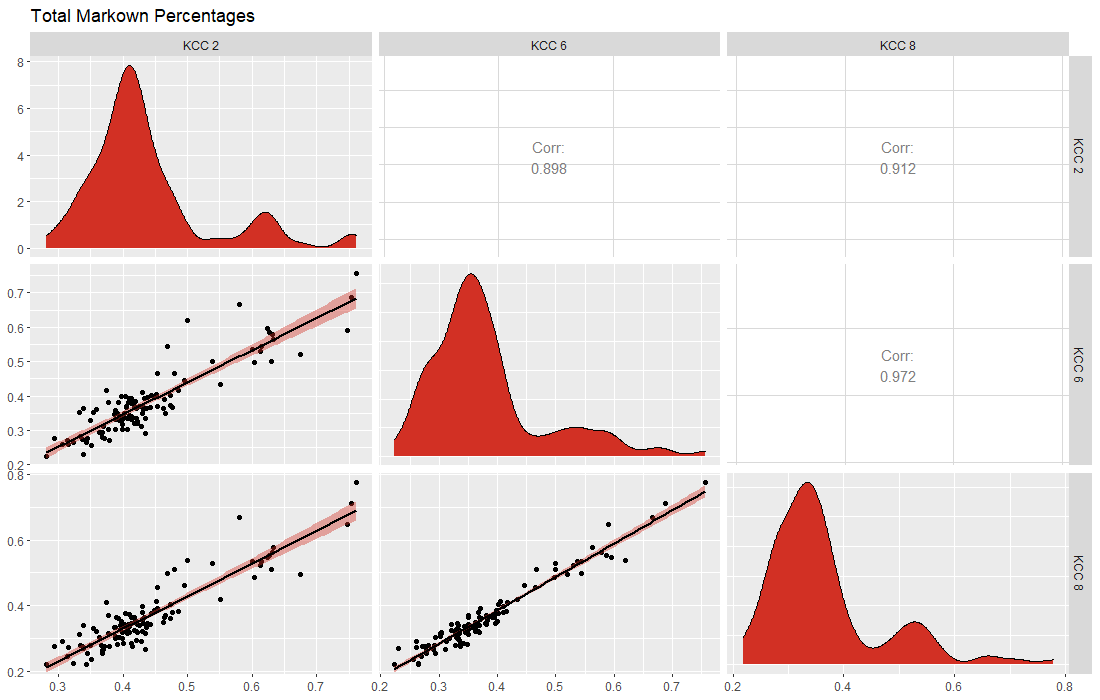
\includegraphics[width=0.9\linewidth]{figures/total_markdown_pct_kcc.png}
  \caption{Pairwise total markdown percentages of the key category clusters (scatterplots, densities \& linear correlations)}
  \label{fig:total_markdown_pct_kcc}
\end{figure}










